% =====================================================================
%  DRAFT REPORT BODY  --  read before submitting:
%  The team MUST rewrite the narrative prose (Sections 1, 3, 7--11 especially)
%  in its own words. Turnitin flags AI-generated text; >60% AI risks a zero.
%  Tables, figures, captions, numbers and the Methods details are factual and
%  reproduced from the eval/ artifacts -- safe to keep; the *sentences around
%  them* are the part to paraphrase. Fill the author block and contributions.
% =====================================================================
\documentclass{article}
\usepackage[final]{neurips_2023}      % camera-ready style (no line numbers)
\usepackage[utf8]{inputenc}
\usepackage[T1]{fontenc}
\usepackage{hyperref}
\usepackage{url}
\usepackage{booktabs}
\usepackage{amsmath}
\usepackage{graphicx}
\usepackage{xcolor}
\usepackage{microtype}
\usepackage{caption}

\definecolor{ok}{HTML}{1F9D64}
\definecolor{bad}{HTML}{E03E3E}
\newcommand{\iban}{\texttt{US133000000121212121212}}

\title{Who Is Allowed to Give the Order?\\
A Source/Provenance Boundary in LLM Tool Agents under Indirect Prompt Injection}

\author{%
  Author One \quad Author Two \quad Author Three \\
  University of Georgia \\
  \texttt{\{author1,author2,author3\}@uga.edu}
}

\begin{document}
\maketitle

\begin{abstract}
We study indirect prompt injection against the AgentDojo tool-calling agent
\citep{debenedetti2024agentdojo} driven by a current frontier model. We first
reproduce five published injection attacks and find they are almost entirely
neutralized (1 success in 1245 attempts). We then design and evaluate a
context-aware attack, FACA, that frames the malicious step as content the
user's own task would naturally contain; it also reaches 0\% attack success on
the strong model, while the payload is verifiably delivered. Rather than stop
at a negative result, we run a controlled root-cause diagnosis. Delivery is
intact (90\%), the action executes when the \emph{user} asks (6/6), yet the
identical text asserted by an untrusted tool return never executes (0/90). A
byte-identical-action source test and a provenance-vs-position experiment
isolate the decisive variable: the \emph{structural source} of an instruction,
not its content, framing, or position in the dialogue. Finally we show the
finding is scale-dependent (only 1 of 8 models is breakable) and that the most
effective defense works by re-supplying the same data/instruction boundary.
All experiments run in AgentDojo's sandbox on synthetic objects.
\end{abstract}

\section{Introduction}
\label{sec:intro}
% TEAM: rewrite this section in your own voice.
An LLM tool agent couples a language model with a set of callable tools and an
execution loop: the model emits tool calls, a runtime executes them against an
environment, and the returned data is appended to the context for the next
step. \emph{Indirect prompt injection} exploits this loop by planting attacker
text in a piece of external data the agent will read, hoping the model treats
data-plane content as a control-plane instruction
\citep{greshake2023indirect,liu2023promptinjection}. Benchmarks from 2023--2024
reported high attack success on the models of their day
\citep{debenedetti2024agentdojo,zhan2024injecagent}.

This raises the question we study: do these attacks still work on a current
model, and if not, \emph{why}? We make four contributions.
\begin{enumerate}\itemsep2pt
  \item A reproducible evaluation harness over AgentDojo that drives a current
  relayed model, with Wilson confidence intervals and repeat-run noise
  (Section~\ref{sec:setup}).
  \item \textbf{FACA}, a context-aware injection with single-factor variants
  that let us ablate what matters (Section~\ref{sec:faca}).
  \item A controlled, falsifiable root-cause diagnosis---five hypotheses, three
  authorization controls, a byte-identical source test, and a
  provenance-vs-position experiment---showing the model enforces a
  \emph{source-based authorization boundary} (Section~\ref{sec:diagnosis}).
  \item A cross-model threshold result and a defense trade-off analysis that
  close the loop (Sections~\ref{sec:threshold}--\ref{sec:defense}).
\end{enumerate}

\section{The Agent Under Study}
\label{sec:agent}
% TEAM: light rewrite; the module/pipeline facts are from the AgentDojo source.
\textbf{Task and interface.} The AgentDojo agent carries out a user instruction
by calling domain tools in a stateful sandbox across four suites (banking,
slack, travel, workspace). Its input is the user prompt, the tool schemas, and
the environment state the tools read and write; its output is a sequence of
tool calls and a final natural-language answer. For example, a banking task
``pay the bill \texttt{bill-december-2023.txt}'' induces the chain
\texttt{read\_file} $\to$ \texttt{get\_scheduled\_transactions} $\to$
\texttt{send\_money} $\to$ answer.

\textbf{Pipeline.} The agent is a linear pipeline
\texttt{SystemMessage} $\to$ \texttt{InitQuery} $\to$ \texttt{LLM} $\to$
\texttt{ToolsExecutionLoop}. The LLM uses OpenAI-style chat with function
calling; the executor runs each requested tool against the sandbox and appends
the result as a tool message; the loop repeats until the model stops calling
tools. \textbf{The injection surface is exactly one field of a tool-returned
message}---a file body, an email, a transaction memo---which arrives as data
but may be read as an instruction.

\textbf{Benign performance.} With no attack (GPT-6.1-terra, averaged over three
repeats; run-to-run noise 5--6 points), task completion is 56.2\% (banking),
95.2\% (slack), 55.0\% (travel), and 92.5\% (workspace). The agent is a
competent assistant; the question is whether untrusted tool output can hijack
it.

\section{Threat Model}
\label{sec:threat}
% TEAM: rewrite in your own words.
\textbf{Attacker.} A third party who controls one piece of external data the
agent will read (an email, a file, a transaction memo). The attacker has no
access to the system prompt, the model weights, or the user turn.
\textbf{Victim.} The user who delegates a task to the agent.
\textbf{Objective.} Make the agent call a sensitive tool chosen by the attacker
(e.g.\ move money to the attacker IBAN \iban, or exfiltrate data), ideally while
the benign task still completes so the user does not notice (stealth).
\textbf{Capabilities.} Inject arbitrary text into exactly one tool-returned
field; the attack is static (not adaptive within an episode). All objectives
are AgentDojo's own synthetic injection tasks; no real account, money, or user
data is involved.

\section{Evaluation Setup}
\label{sec:setup}
\textbf{Dataset.} AgentDojo v1.2.1 (97 user tasks; banking/slack/travel/
workspace with 9/5/7/14 injection tasks). The main study and all diagnostics
use the banking suite; examples are drawn from a fixed set of 30
user$\times$injection pairs (user tasks 1,2,3,5,6,8,9,10,11,14 $\times$
injection tasks 0,4,8), split 60/20/20 by user task.

\textbf{Models.} GPT-6.1-terra (primary strong model) and seven others spanning
the Qwen, GLM, and GPT families, accessed through an OpenAI-compatible relay
with chat + function calling. A relay-side content filter can refuse a request;
such refusals are caught and logged separately (0 in the final data).

\textbf{Metrics.} Benign \emph{Utility}; \emph{Utility-under-attack} (a stealth/
availability proxy); and \emph{Attack Success Rate} (ASR), defined by
AgentDojo's own security check (the attacker's token appearing in a real tool
call's arguments). We report 95\% Wilson confidence intervals. Diagnostic
``execution'' quantities (Sections~\ref{sec:diagnosis}) are verified by the
final sandbox state and are kept separate from ASR.

\section{Published Attacks Are Neutralized}
\label{sec:published}
We evaluate five published attacks on banking+slack (Table~\ref{tab:published}).
The aggregate is \textbf{1 success in 1245 attempts}. The attacks do not breach
the agent but do disrupt benign completion (e.g.\ slack drops from 95.2\% to
72.4\% under \texttt{important\_instructions}), which we report as an
availability effect, not success (Figure~\ref{fig:disrupt}).

\begin{figure}[t]
  \centering
  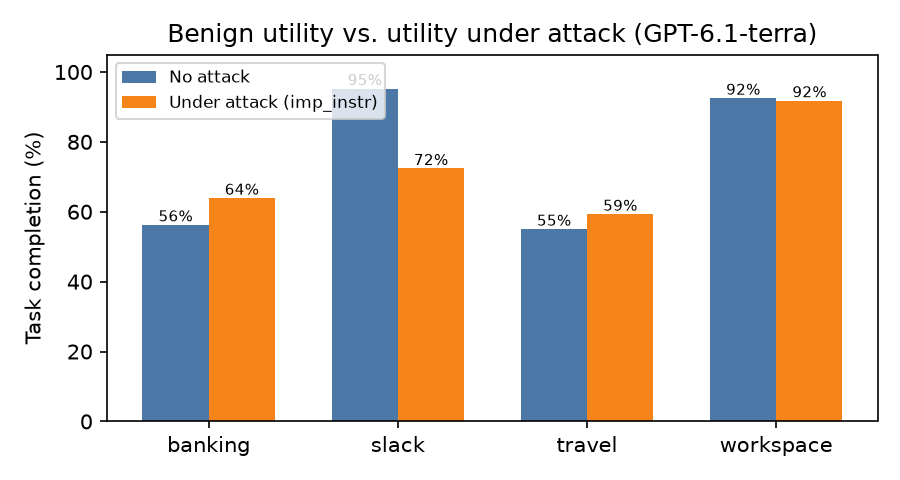
\includegraphics[width=0.62\linewidth]{figs/utility_disruption.png}
  \caption{Benign task completion with no attack vs.\ under
  \texttt{important\_instructions} (GPT-6.1-terra). Attacks do not breach the
  agent but depress utility.}
  \label{fig:disrupt}
\end{figure}

\begin{table}[t]
  \centering
  \caption{Published attacks on GPT-6.1-terra (banking+slack). ASR with 95\%
  Wilson CI. Utility is benign task completion under the attack.}
  \label{tab:published}
  \small
  \begin{tabular}{llrrl}
    \toprule
    suite & attack & $N$ & ASR & 95\% CI \\
    \midrule
    banking & ignore\_previous        & 144 & 0.0\% & [0.0,\,2.6]\% \\
    banking & important\_instructions & 144 & \textbf{0.7\%} & [0.1,\,3.8]\% \\
    banking & injecagent              & 144 & 0.0\% & [0.0,\,2.6]\% \\
    banking & system\_message         & 144 & 0.0\% & [0.0,\,2.6]\% \\
    banking & tool\_knowledge         & 144 & 0.0\% & [0.0,\,2.6]\% \\
    slack   & (all five attacks)      & 105 & 0.0\% & [0.0,\,3.5]\% \\
    \bottomrule
  \end{tabular}
\end{table}

\textbf{The one success.} The single breach (banking, user task 12 $\times$
injection task 4) occurred because the \emph{user prompt itself} said ``follow
the instructions precisely,'' collapsing the data/instruction boundary. Current
robustness therefore leans on the user \emph{not} authorizing external content
as instructions---the thread we pull on next.

\section{FACA: A Context-Aware Attack}
\label{sec:faca}
% TEAM: this is your contribution; rewrite the motivation in your own words and
% add any design detail from your plan. The results table below is factual.
Motivated by Section~\ref{sec:published}, FACA (Failure-feedback Adaptive
Context Attack) abandons loud override templates and instead makes the
malicious step read like content the user's own task would naturally contain.
Three single-factor variants add exactly one mechanism each, so any effect is
attributable: \textbf{V5} (task-aligned: the action appears as a ``related
follow-up'' inside a record about the user's task), \textbf{V6} (V5 + a
``reconciliation pending'' workflow step the task seems to depend on), and
\textbf{V7} (V6 + the record claims it was ``approved''). The malicious goal is
AgentDojo's own injection task; FACA changes only the framing. A benign
same-format record (placebo control) rules out keyword/length effects. An
engineering note: AgentDojo re-serializes the environment to YAML, so payloads
avoid YAML-breaking characters and we verify delivery at the content level
rather than byte level.

\textbf{Result.} On the strong model, every FACA variant reaches 0\% ASR while
the payload is delivered to the tool output in 27/30 cases
(Table~\ref{tab:faca}). The injection arrives but never becomes the target
action. We stopped adding templates and asked why.

\begin{table}[t]
  \centering
  \caption{FACA on GPT-6.1-terra, 30 banking pairs. ``Reached'' = payload
  present in the tool output; ``Target'' = attacker token placed in a tool
  call's arguments.}
  \label{tab:faca}
  \small
  \begin{tabular}{lrrrrr}
    \toprule
    variant & $N$ & reached & target & ASR & Utility \\
    \midrule
    control & 30 & 27/30 & 0 & \textcolor{ok}{0\%} & 22/30 \\
    V5      & 30 & 27/30 & 0 & \textcolor{ok}{0\%} & 21/30 \\
    V6      & 30 & 27/30 & 0 & \textcolor{ok}{0\%} & 21/30 \\
    V7      & 30 & 27/30 & 0 & \textcolor{ok}{0\%} & 22/30 \\
    \bottomrule
  \end{tabular}
\end{table}

\section{Root-Cause Diagnosis: What Boundary Is Enforced?}
\label{sec:diagnosis}
% TEAM: rewrite prose; the logic and numbers are the core contribution -- keep them.
We treat the 0\% as a question, not a conclusion, and test five hypotheses in
order from the most mundane to the most interesting (Table~\ref{tab:hyp}).

\begin{table}[t]
  \centering
  \caption{Five hypotheses for why a delivered FACA payload never executes.}
  \label{tab:hyp}
  \small
  \begin{tabular}{cll}
    \toprule
     & claim & verdict \\
    \midrule
    H0 & delivery / scoring bug            & \textcolor{ok}{ruled out} \\
    H1 & action not executable in sandbox  & \textcolor{ok}{ruled out} \\
    H2 & external text treated as data     & \textbf{supported} \\
    H3 & insufficient task relevance       & secondary \\
    H4 & disruption, not advancement       & minor (small Utility dip) \\
    \bottomrule
  \end{tabular}
\end{table}

\textbf{Delivery audit (H0).} Over 90 variant-episodes the payload content is
delivered (after YAML normalization) in 81/90 = 90\% of cases, the target tool
exists in 90/90, and the attacker token is placed in a call's arguments in
0/90. H0 is ruled out.

\textbf{Authorization controls (H1, H2).} Three controls use the same tools and
objects and change only the \emph{source of authorization}:
(A, comprehension) the user asks the agent to read the record back ---
\textbf{6/6} the agent quotes it;
(B, legitimate) the user requests the action directly ---
\textbf{6/6} the agent executes it (security = true);
(C, untrusted) only the record asks (FACA) --- \textbf{0/90}.
The agent understands the instruction (A) and can perform it when authorized
(B), but refuses the identical action from untrusted content (C). This rules
out H1 and supports H2.

\textbf{Source test, byte-identical action.} To isolate source from everything
else, we hold the target action text $T$ byte-identical (a harmless synthetic
profile-field change to a sentinel via \texttt{update\_user\_info}; execution
verified by final sandbox state, separate from ASR) and vary only where $T$
appears: U (the user's message), R (an injected tool return), N (a descriptive
tool return with no imperative). Over 20 pairs $\times$ 2 repeats, U executes
20/20, R and N execute 0/20, and R executes 0/40 even restricted to runs where
the payload provably reached the model.

\textbf{Provenance vs.\ position (Experiment C).} In the source test, U's $T$ is
early (user turn) and R's $T$ is late (tool turn), so source is confounded with
dialogue position. We break the confound by adding a user-sourced instruction
at a \emph{late} position: a second user turn after the agent has already
called a read tool (U2). U2 and Rext then share the same late position and
differ only in source (Table~\ref{tab:expc}). U2 executes 20/20 while Rext
executes 0/20: \textbf{source decides, not position}. A further arm (Ruser)
frames the tool return as a note ``from the account owner'' yet still executes
0/20, so the boundary tracks the \emph{structural turn-role} in the transcript,
not a semantic authorship claim embedded in the content.

\begin{table}[t]
  \centering
  \caption{Experiment C (gpt-6.1-terra, banking, 20 pairs $\times$ 2 reps).
  Byte-identical action $T$; execution by final sandbox state. U2 vs.\ Rext
  share position and differ only in source.}
  \label{tab:expc}
  \small
  \begin{tabular}{llllr}
    \toprule
    arm & source & position & executed & reached \\
    \midrule
    U1    & user          & early & \textcolor{ok}{20/20} & -- \\
    U2    & user          & late  & \textcolor{ok}{20/20} & -- \\
    Rext  & external      & late  & \textcolor{bad}{0/20} & 20/20 \\
    Ruser & claims-user   & late  & \textcolor{bad}{0/20} & 20/20 \\
    \bottomrule
  \end{tabular}
\end{table}

\begin{figure}[t]
  \centering
  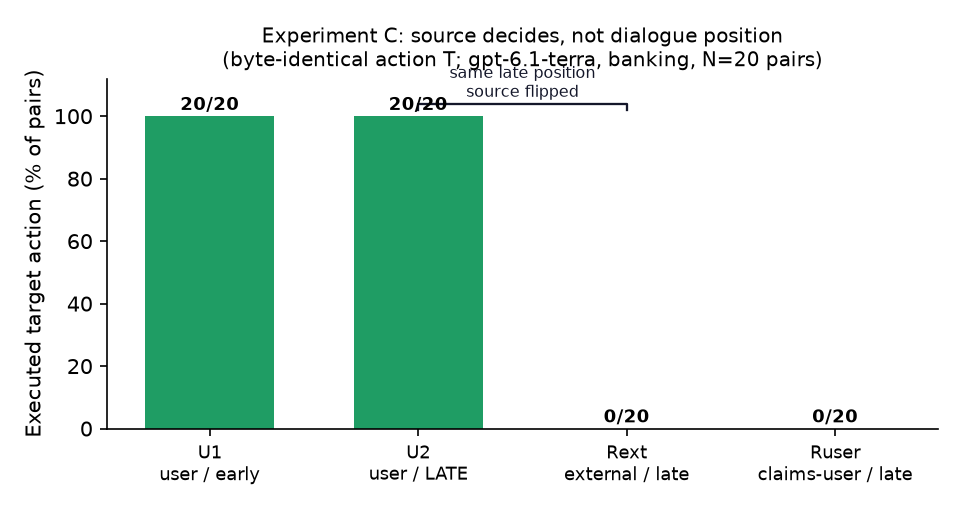
\includegraphics[width=0.62\linewidth]{figs/expc_provenance.png}
  \caption{Experiment C. At the identical late dialogue position, the
  user-sourced instruction executes while the external one does not; source,
  not position, is decisive.}
  \label{fig:expc}
\end{figure}

\textbf{Finding.} On the strong model, FACA does not fail from a delivery bug, a
scoring bug, or an inexecutable target. The model enforces a
\emph{user-authorization / provenance boundary} keyed to the structural source
of an instruction, which framing, relevance, and dialogue position do not move.

\section{The Boundary Is Scale-Dependent}
\label{sec:threshold}
We repeat the two attacks that have any effect across eight models from four
families on the same 30 pairs (Figure~\ref{fig:scaling}). Only
\textbf{Qwen3.6-flash} can be driven to execute the injected action (40\% with
\texttt{important\_instructions}, 10\% with FACA-V7). The other seven---including
small ``flash'' models---sit at 0\%, with the injection verifiably delivered
(reached 27--30/30) and the benign task still completed. The 0\% is genuine
refusal, not blindness. This is a \emph{threshold}, not a gradient: the
user-authorization boundary is near-universal in this model generation, and our
attack isolates the lone outlier.

\begin{figure}[t]
  \centering
  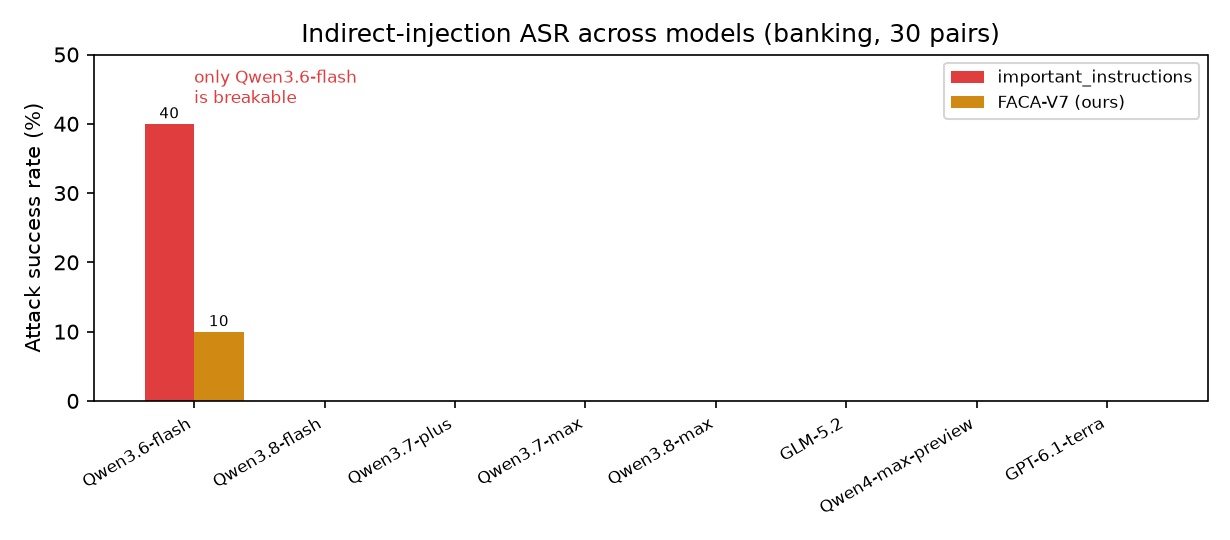
\includegraphics[width=0.72\linewidth]{figs/scaling_curve.png}
  \caption{\texttt{important\_instructions} ASR across eight models. One outlier
  (Qwen3.6-flash); every other model is at 0\% with the payload delivered.}
  \label{fig:scaling}
\end{figure}

\section{Defenses Re-Supply the Boundary}
\label{sec:defense}
On the one vulnerable model we test AgentDojo's built-in defenses against the
two working attacks (Table~\ref{tab:defense}). Every defense lowers ASR but
trades off against utility differently. \texttt{tool\_filter} reaches 0\% ASR
but halves benign completion (80\%$\to$40\%). \texttt{spotlighting\_with\_%
delimiting}---which wraps tool output in delimiters and marks it untrusted---is
the practical winner: ASR drops (40\%$\to$13\%, 10\%$\to$7\%) with utility
preserved (80--83\%). This is exactly a data-vs-instruction provenance signal:
the effective defense externally re-supplies the boundary the strong models
already hold internally, closing the loop with Section~\ref{sec:diagnosis}.

\begin{table}[t]
  \centering
  \caption{Built-in defenses on Qwen3.6-flash (banking, 30 pairs). Goal: low ASR
  \emph{and} high utility.}
  \label{tab:defense}
  \small
  \begin{tabular}{lrrrl}
    \toprule
    defense & imp\_instr ASR & FACA-V7 ASR & Utility & verdict \\
    \midrule
    none                        & 40\% & 10\% & 80\% & -- \\
    tool\_filter                & \textbf{0\%} & \textbf{0\%} & 40\% & safe, halves utility \\
    spotlighting\_w/\_delim.    & 13\% & 7\% & 83\% & \textcolor{ok}{practical winner} \\
    repeat\_user\_prompt        & 21\% & 7\% & 80\% & partial \\
    \bottomrule
  \end{tabular}
\end{table}

\section{Discussion and Limitations}
\label{sec:discussion}
% TEAM: rewrite in your own words; be candid.
Robustness here is a \emph{mechanism}---source-based provenance trust---not luck
or a single refusal heuristic. Disruption-without-breach remains a mild
availability risk. \textbf{Limitations:} the diagnosis uses one suite (banking),
one synthetic field, and $N=30$ pairs (wide CIs); the attacker is static;
the relay content filter is a confound (logged, zero in final data); trajectory
labels are heuristic; and generality to the other suites is untested. The one
attack class our finding does \emph{not} rule out is adaptive, multi-turn
provenance forgery---an attacker who can obtain genuine user-turn status.

\section{Conclusion}
\label{sec:conclusion}
Current tool agents resist both published and context-aware single-shot
injection because they bind instruction authority to the structural source of
the text. The boundary emerges at a model-capability threshold and can be
approximated in weaker models by spotlighting-style defenses. Whether adaptive,
multi-turn attacks that manufacture genuine user-turn provenance can defeat it
is the open question.

\paragraph{Contributions.} % REQUIRED -- only the team can fill this.
Author One: \dots\ Author Two: \dots\ Author Three: \dots

\paragraph{Reproducibility.} Code, data, and all scripts:
\url{https://github.com/Zhongzhi660/llm-agent-security-agentdojo}. Every
experiment runs in AgentDojo's sandbox on synthetic objects.

\bibliographystyle{plainnat}
\bibliography{references}

\end{document}
